%==============================================================================
% Sjabloon poster bachproef
%==============================================================================
% Gebaseerd op document class `a0poster' door Gerlinde Kettl en Matthias Weiser
% Aangepast voor gebruik aan HOGENT door Jens Buysse en Bert Van Vreckem

\documentclass[a0,portrait]{hogent-poster}




\usepackage[most]{tcolorbox}
\usepackage{xcolor}

% Aanpasbare kleuren
\definecolor{titlecolor}{RGB}{76,162,213}
\definecolor{bordercolor}{RGB}{76,162,213}
\definecolor{boxbackground}{RGB}{255,255,255}

\newtcolorbox{posterbox}[1]{
    enhanced,
    colback=boxbackground,
    colframe=bordercolor,
    boxrule=0.8pt,
    arc=2mm,
    left=3mm,
    right=3mm,
    top=4mm,
    bottom=2mm,
    title={#1},
    coltitle=white,
    colbacktitle=titlecolor,
    fonttitle=\bfseries\large,
    toptitle=1.5mm,
    bottomtitle=1.5mm,
    lefttitle=3mm,
    righttitle=3mm,
    sharp corners=north
}

% Info over de opleiding
\course{Bachelorproef}
\studyprogramme{toegepaste informatica}
\academicyear{2025-2026}
\institution{Hogeschool Gent, Valentin Vaerwyckweg 1, 9000 Gent}

% Info over de bachelorproef
\title{Ontwerp en realisatie van een performante provisioner voor virtuele Windows-en Linux omgevingen in Rust.}
\author{Jens Gosseye}
\email{jens.gosseye@student.hogent.be}
\supervisor{Dhr. B. Van Vreckem}
\cosupervisor{Dhr. J. Courtens (HOGENT)}
% Indien ingevuld, wordt deze informatie toegevoegd aan het einde van de
% abstract. Zet in commentaar als je dit niet wilt.
\specialisation{Systeem- en Netwerkbeheer}
\keywords{Rust, Virtualbox, Windows, Linux}
\projectrepo{https://github.com/JensGos/BP_Rust_Provision}

\begin{document}

\maketitle

\begin{abstract}
Deze bachelorproef onderzoekt RustProv, een provisioner in Rust voor virtuele Linux- en Windowsomgevingen. De tool automatiseert het opstarten, configureren en provisionen van één of meerdere virtuele machines via TOML-configuratie en SSH. RustProv werd vergeleken met Vagrant in Linux- en Windowsscenario's. De resultaten tonen aan dat RustProv vooral bij meerdere VM's sneller is dan Vagrant.
\end{abstract}

\begin{multicols}{2} % This is how many columns your poster will be broken into, a portrait poster is generally split into 2 columns

\begin{posterbox}{1. Probleemstelling \& Onderzoeksvraag}

\textbf{Huidige situatie en Probleem} \\
Binnen de opleiding Toegepaste Informatica aan HOGENT wordt Vagrant gebruikt om virtuele Windows- en Linuxomgevingen automatisch op te zetten. In de praktijk zorgen deze omgevingen echter regelmatig voor de volgende problemen:

\begin{itemize}
    \item Virtuele machines starten soms traag op.
    \item Het provisioningproces kan vastlopen of door time-outs worden onderbroken.
    \item Bij meerdere virtuele machines loopt de wachttijd sterk op.
    \item Een onderbroken provisioningproces kan op de achtergrond blijven draaien.
    \item Studenten en lectoren verliezen hierdoor tijd tijdens labo's, oefeningen en evaluaties.
\end{itemize}

\textbf{Onderzoeksvraag}
\begin{quote}
    \textit{Hoe ontwerp en realiseer je een performante provisioner voor virtuele Windows- en Linuxomgevingen die beter inspeelt op de behoeften van onderwijs- en labo-omgevingen dan de huidige Vagrant-gebaseerde aanpak?}
\end{quote}

\textbf{Doelstelling en Scope} \\
RustProv is ontwikkeld als een proof of concept in Rust. De tool moet:

\begin{itemize}
    \item Windows- en Linux-VM's kunnen opstarten en provisionen.
    \item Eén of meerdere VM's kunnen beheren.
    \item Configuratie uit een leesbaar TOML-bestand kunnen inlezen.
    \item Provisioningscripts via SSH kunnen uitvoeren.
    \item VM-statussen, snapshots en foutscenario's kunnen beheren.
    \item De provisioningstijd ten opzichte van Vagrant kunnen verkorten.
\end{itemize}

De centrale focus ligt dus niet alleen op het aanmaken van VM's, maar vooral op het volledig geautomatiseerd opstarten, bereiken en provisionen van een bruikbare omgeving.
\end{posterbox}

\definecolor{titlecolor}{RGB}{65,138,181}
\definecolor{bordercolor}{RGB}{65,138,181}
\definecolor{boxbackground}{RGB}{255,255,255}

\begin{posterbox}{2. Methodologie}
    
\centering
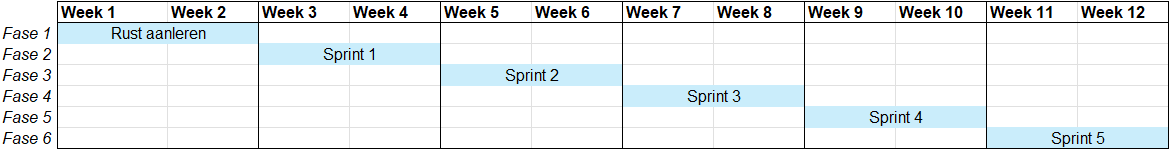
\includegraphics[
width=\linewidth,
keepaspectratio
]{img/Gantt Diagram.png}
\captionof{figure}{Gantt diagram met de verschillende fasen.}

\vspace{4mm}
\raggedright

\textbf{Rust leren \& onderzoek:}\\
- Rust, virtualisatie en provisioning verkennen; vereisten bepalen.

\vspace{1.5mm}

\textbf{Sprint 1 -- Opstarten:}\\
- VM's aanmaken, configureren en starten in VirtualBox.

\vspace{1.5mm}

\textbf{Sprint 2 -- Provisionen:}\\
- Via SSH scripts uitvoeren op Linux- en Windows-VM's.

\vspace{1.5mm}

\textbf{Sprint 3 -- Configuratie:}\\
- VM-instellingen inlezen vanuit TOML.

\vspace{1.5mm}

\textbf{Sprint 4 -- Uitbreidingen:}\\
- Snapshots, statuscontrole en meerdere VM's.

\vspace{1.5mm}

\textbf{Sprint 5 -- Robuustheid:}\\
- Prioriteiten, foutafhandeling en noodfuncties.
    
\end{posterbox}


\definecolor{titlecolor}{RGB}{53,113,149}
\definecolor{bordercolor}{RGB}{53,113,149}
\definecolor{boxbackground}{RGB}{255,255,255}


\begin{posterbox}{3. Functionaliteiten}

RustProv beheert virtuele machines via een command-line interface en een extern
TOML-configuratiebestand.

\vspace{0.5cm}

\noindent
\begin{minipage}[t]{0.48\columnwidth}
    \centering
    \scriptsize
    \begin{verbatim}
        Commands:
        start      Start VM(s)
        stop       Stop VM(s)
        provision  Provision VM(s)
        state      Check VM state
        remove     Remove VM(s)
        restore    Restore snapshot(s)
        ssh        SSH into a VM
        kill       Kill VirtualBox
        init       Initialize tool
    \end{verbatim}
    
    \captionof{figure}{RustProv commando's.}
\end{minipage}%
\hfill
\begin{minipage}[t]{0.48\columnwidth}
    \centering
    \scriptsize
    \begin{verbatim}
        [linuxbp]
        image = "almalinux9"
        cores = 4
        memory = 4096
        script = ["00-hello.sh"]
        bridgeNetwork = 
        "Realtek Gaming 2.5GbE 
        Family Controller"
    \end{verbatim}
    
    \captionof{figure}{Voorbeeld TOML-config.}
\end{minipage}
\end{posterbox}


\definecolor{titlecolor}{RGB}{42,89,117}
\definecolor{bordercolor}{RGB}{42,89,117}
\definecolor{boxbackground}{RGB}{255,255,255}

\begin{posterbox}{4. Resultaten}

RustProv werd vergeleken met Vagrant in vier testscenario's: één Linux-VM, drie Linux-VM's, één Windows-VM en drie Windows-VM's. De Linuxomgeving bestond uit een serveropstelling met onder andere WordPress, Loki en Grafana. De Windowsomgeving bestond uit een Active Directory-omgeving met twee servers en één client.

\begin{center}
    \begin{tabular}{lrr}
        \hline
        \textbf{Scenario} & \textbf{Snellere tool} & \textbf{Tijdsverschil} \\
        \hline
        Eén Linux-VM & Vagrant & 2,35 s \\
        Drie Linux-VM's & RustProv & 74,03 s \\
        Eén Windows-VM & RustProv & 58,91 s \\
        Drie Windows-VM's & RustProv & 472,10 s \\
        \hline
    \end{tabular}
\end{center}
\end{posterbox}

\definecolor{titlecolor}{RGB}{30,65,85}
\definecolor{bordercolor}{RGB}{30,65,85}
\definecolor{boxbackground}{RGB}{255,255,255}

\begin{posterbox}{5. Conclusie \& Toekomst}
    
De Proof of Concept toont aan dat RustProv virtuele Linux- en Windowsomgevingen automatisch kan opstarten en provisionen. In de meeste testscenario's was RustProv sneller dan Vagrant. De grootste tijdswinst werd gemeten bij het provisionen van meerdere VM's.

De resultaten tonen aan dat RustProv vooral geschikt is voor onderwijs- en labo-omgevingen waar regelmatig dezelfde VM-opstellingen moeten worden opgebouwd. Door de TOML-configuratie en de ondersteuning voor meerdere VM's kunnen deze omgevingen reproduceerbaar worden opgezet.

\textbf{Toekomstig onderzoek \& optimalisatie:}

\begin{itemize}
    \item \textbf{Parallel provisionen:} onafhankelijke VM's gelijktijdig configureren om de totale uitvoeringstijd verder te verkorten.
    \item \textbf{Uitbreiding:} provisioningscripts uitvoeren op fysieke machines, naast virtuele machines.
    \item \textbf{Betrouwbaarheid:} logging, foutmeldingen en automatische herstelacties verder verbeteren.
    \item \textbf{Gebruiksgemak:} een grafische interface, installatieprocedure en uitgebreidere gebruikershandleiding toevoegen.
\end{itemize}
\end{posterbox}
    

\end{multicols}
\end{document}